\documentclass[unknownkeysallowed]{beamer}
\usetheme{Madrid}
\usepackage{subfig}
\usepackage{xcolor}
\usepackage{wrapfig}
\usepackage[utf8]{inputenc}
\usepackage[polish]{babel}
\usepackage[T1]{fontenc}
\usepackage[]{algorithm2e}

\title{Gradient Naturalny}
\subtitle{}
\author{Jakub Bartczuk}
\centering
\date{Kwiecień 2020}
\makeatletter
\renewcommand{\@algocf@capt@plain}{above}% formerly {bottom}
\makeatother
\begin{document}
\maketitle

% macros
\newcommand{\gradfx}{\nabla f(x)}
\newcommand{\gradloglikelihood}[1]{\nabla_{\theta} log p_{\theta}(#1)}
\newcommand{\naturalgrad}{\widetilde{\nabla}_{\theta}J}
\newcommand{\fisher}{\mathbf{F}}
\begin{frame}{Gradient Descent}
  Minimalizujemy różniczkowalną funkcję $f$.

  Przybliżenie szeregiem Taylora pierwszego rzędu daje
  $$f(x + \delta) \approx g(x) = f(x) + \gradfx^T \delta $$

  Minimalizacja g sugeruje procedurę 
  $$x_{t+1} = x_t - \alpha \nabla f(x_t)$$

  $\alpha$ znajdujemy line searchem

\end{frame}

\begin{frame}{Problemy z GD}
  Metoda nie jest niezmiennicza względem reparametryzacji: zbieżność zależy od wartości własnych Hesjanu
    \begin{columns}

        \column{.5\textwidth}
        \begin{center}$f(x,y ) = x^2 + y^2$\end{center}
        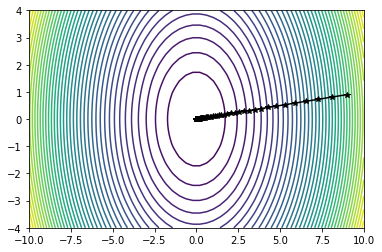
\includegraphics[width=\textwidth]{GD1.png} 
        \column{.5\textwidth}
        \begin{center}$f(x,y ) = x^2 + 10 y^2$\end{center}
        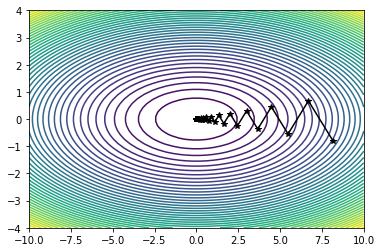
\includegraphics[width=\textwidth]{GD10.png} 
    \end{columns}
\end{frame}

\begin{frame}{Metody Spadku (Steepest descent)}
  Powyższą procedurę można zinterpretować tak: dla zadanej normy $\| \|$

  $$\Delta x_{nsd} = argmin_v \{\gradfx v : \|v\| = 1 \}$$ 
  $$f(x + \delta) \approx g(x) = f(x) + \gradfx^T \delta $$
  
  Szukanie $\Delta x_{nsd}$ z różnych norm $\|x\| = \|Px\|_2$ jest równoważne optymalizacji spadkiem gradientu funkcji $h(x) = f(P^{1/2}x)$ \pause
  

  Intuicyjne jest żeby zmienić parametryzację tak, aby uwarunkowanie Hesjanu było równe 1.
  \begin{block}{Metoda Newtona}
  $$x_{t+1} = x_t - H_f(x)^{-1} \nabla f(x_t)$$
  \end{block}

\end{frame}

\begin{frame}{Wypukłość}
  Powyższe metody zakładały wypukłość 

  Przykład: Hesjan który nie jest dodatnio określony (start w punkcie siodłowym)

 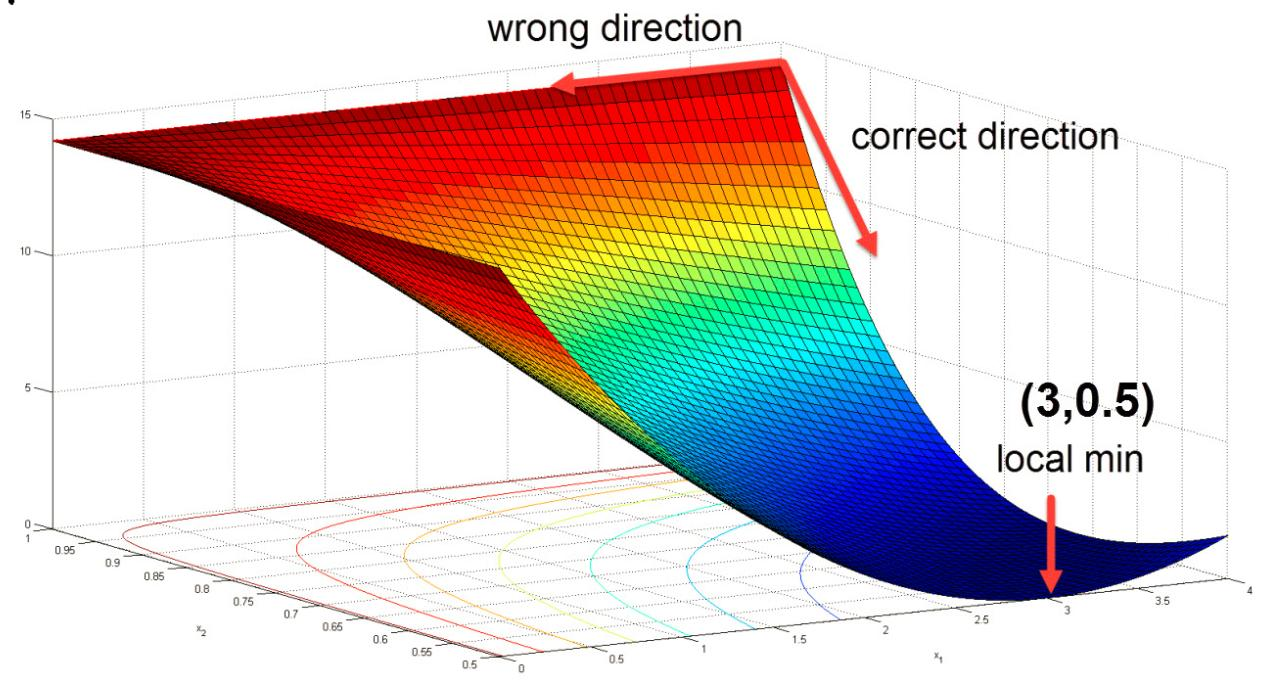
\includegraphics[width=\textwidth]{Niewypukla.jpg} 
\end{frame}

\begin{frame}{Co wspólnego mają powyższe metody}
  \begin{block}{Metody spadku}
  Zakładamy, że $\delta$ jest małe tzn $\| \delta \| < \epsilon$
  Przybliżamy $f(x + \delta)$
  \end{block}

  \begin{block}{Gradient naturalny}
    $\theta$ parametryzuje rodzinę rozkładów $p_{\theta}$

    $$J(\theta) = \mathbb{E}_{x \sim p_{\theta}}[c(x)]$$

    Minimalizujemy $J(\theta)$ za pomocą $p_{\theta + \delta}$ bliskiego w sensie KL-dywergencji
  \end{block}
\end{frame}


\begin{frame}{Gradient Naturalny}
  \begin{block}{GN dokładniej}
    Szukamy $\delta$
    $$\underset{\delta: KL(p_{\theta + \delta} || p_{\theta}) < \epsilon}{argmin} J(\theta + \delta)$$ \pause
    $$J(\theta + \delta) \approx g(\theta) = J(\theta) + \nabla J(\theta)^T \delta $$ \pause

    \end{block}
    \begin{block}{Mnożniki Lagrange'a - $g$ i przybliżenie Taylora $KL$ dywergencji
}
 
    $$\mathcal{L}(\theta, \delta, \beta) = J(\theta) + \nabla J(\theta)^T \delta - \beta(\frac{1}{2}\delta^T \fisher \delta + \epsilon) = 0$$
    $$\nabla_{\delta} \mathcal{L}(\theta, \delta, \beta) = \nabla J(\theta)  - \beta \fisher \delta = 0$$\pause
    Czyli
    $$\naturalgrad =_{def} \delta^*  = \fisher^{-1} \nabla J(\theta)$$
     
    \end{block}
    \end{frame}

\begin{frame}{Informacja Fishera}
      \begin{block}{Przybliżenie KL-dywergencji}
    $$KL(p_{\theta + \delta} || p_{\theta}) = \mathbb{E}_{x \sim p_{\theta}}[log p_{\theta}(x) - log p_{\theta + \delta}(x)] \approx$$
    $$\mathbb{E}_{x \sim p_{\theta}}[log p_{\theta}(x) - (log p_{\theta}(x) + \gradloglikelihood{x}^T \delta+ \frac{1}{2} \delta^T \gradloglikelihood{x}\gradloglikelihood{x}^T \delta )] = $$
    $$\mathbb{E}_{x \sim p_{\theta}}[- \gradloglikelihood{x}^T \delta -\frac{1}{2} \delta^T \gradloglikelihood{x}\gradloglikelihood{x}^T \delta )] =$$ \pause
    $$ -\frac{1}{2}\delta^T \mathbb{E}_{x \sim p_{\theta}}[ \gradloglikelihood{x}\gradloglikelihood{x}^T  )] \delta = -\frac{1}{2}\delta^T \fisher \delta$$

    $\fisher$ jest nazywana \textbf{Macierzą Informacji Fishera}
  \end{block}

\end{frame}

    
\begin{frame}{Natural Evolution Strategies}
% formerly {bottom}
  \begin{algorithm}[H]
\caption{Natural Evolution Strategies}
 \KwData{f, $\theta_{init}$}
 \While{not converged}{
   \For{k in [1, .. $\lambda$]}{
     $z_k = sample(p_{\theta})$\;
   }
   $\nabla_{\theta}J = \frac{1}{\lambda} \underset{k < \lambda}{\sum} f(z_k) \gradloglikelihood{z_k}$\;
   $F = \frac{1}{\lambda} \underset{k < \lambda}{\sum} \gradloglikelihood{z_k}\gradloglikelihood{z_k}^T$\;
   $\naturalgrad = F^{-1} \nabla_{\theta}J$\;
   $\theta = \theta - \alpha \naturalgrad $
 }
\end{algorithm}  
\end{frame}

\begin{frame}{Uwagi}
  \begin{itemize}
  \item powyższy algorytm stosuje się dla funkcji $f$ pochodzącej od optymalizowanej funkcji \pause
  \item różne prace teoretyczne pokazują równoważność algorytmu NES z CMA-ES (np \textit{Bidirectional Relation between CMA Evolution Strategies and Natural Evolution Strategies}) 
  \end{itemize}

\end{frame}
\end{document}